\documentclass[10pt]{article}
\usepackage{amsmath,amssymb,theorem}
\usepackage{caption}
\usepackage{tikz}
\usetikzlibrary{arrows.meta, automata, positioning, quotes}
\usepackage{graphicx}
\textwidth = 6.5 in
\textheight = 9 in
\oddsidemargin = 0.0 in
\evensidemargin = 0.0 in
\topmargin = 0.0 in
\headheight = 0.0 in
\headsep = 0.0 in
\parskip = 0.2in
\parindent = 0.0in
\DeclareGraphicsExtensions{.pdf, .jpg, .png}

\begin{document}
\begin{figure}[h]
    \centering
    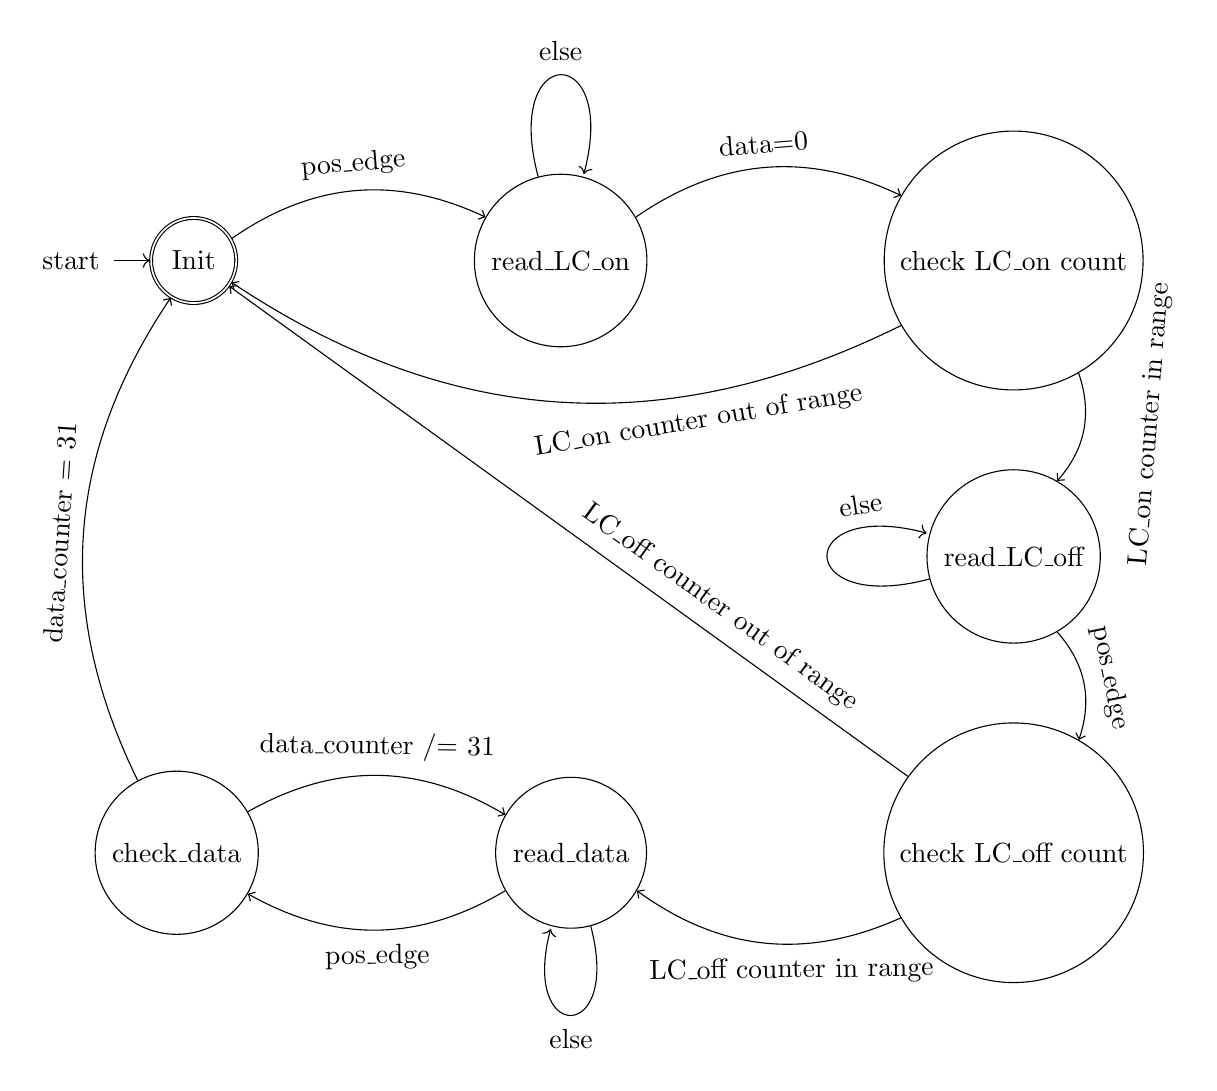
\begin{tikzpicture}
        [
        node distance = 10mm and 30 mm,
        inner sep=5pt,
        every edge/.append style = {draw, -{Straight Barb[scale=0.8]}},
        every edge quotes/.style = {auto=center, font=\small, inner sep=6pt}
        ]
        % nodes
        \node[state, initial, accepting] (1) {Init};
        \node[state, right= of 1] (2) {read\_LC\_on};
        \node[state, right= of 2] (3) {check LC\_on count};
        \node[state, below= of 3] (4) {read\_LC\_off};
        \node[state, below= of 4] (5) {check LC\_off count};
        \node[state, left= of 5] (6) {read\_data};
        \node[state, left= of 6] (7) {check\_data};
        % arrows
        \path [every node/.style={sloped,above}]
        (1) edge[bend left] node {pos\_edge} (2)
        (2) edge[loop above] node {else} ()
        edge[bend left] node {data=0} (3)
        (3) edge[bend left] node [pos=.3,below]{LC\_on counter out of range} (1)
        edge[bend left] node [below=14pt,pos=.4]{LC\_on counter in range} (4)
        (4) edge[loop left] node [pos=.8]{else} ()
        edge[bend left] node {pos\_edge} (5)
        (5) edge node [pos=.3]{LC\_off counter out of range} (1)
        edge[bend left] node [below,pos=.4]{LC\_off counter in range} (6)
        (6) edge[bend left] node [below]{pos\_edge}(7)
        edge[loop below] node [below]{else} ()
        (7) edge[bend left] node {data\_counter /= 31} (6)
        edge[bend left] node {data\_counter = 31} (1);
    \end{tikzpicture}
    \caption{State Diagram for the Remote Controller}
    \label{fig:my_label}
\end{figure}
\end{document}